\documentclass{article}

\usepackage{array}
\usepackage{booktabs}
\usepackage{multirow}
\newcommand{\head}[1]{\textnormal{\textbf{#1}}}
\newcommand{\normal}[1]{\multicolumn{1}{l}{#1}}

\usepackage{enumitem}
\usepackage[square]{natbib}
\usepackage{tocloft}

\usepackage{amsmath}
\let\oldFootnote\footnote
\newcommand\nextToken\relax

\renewcommand\footnote[1]{%
    \oldFootnote{#1}\futurelet\nextToken\isFootnote}

\newcommand\isFootnote{%
    \ifx\footnote\nextToken\textsuperscript{,}\fi}
    
\usepackage[utf8]{inputenc}
\usepackage[T1]{fontenc}
\usepackage{lmodern}
\usepackage[french]{babel}
\usepackage{float}
\usepackage[table]{xcolor}
\usepackage{graphicx}
\usepackage{fontawesome}

\usepackage{tikz}
\let\svtikzpicture\tikzpicture
\def\tikzpicture{\noindent\svtikzpicture}

\makeatletter
\def\input@path{{../src/}}
\makeatother

\setlength{\cftbeforepartskip}{18pt}

\renewcommand{\cftsecleader}{\cftdotfill{\cftdotsep}}

\usepackage{titlesec}

\setcounter{secnumdepth}{4}

\titleformat{\paragraph}
{\normalfont\small\bfseries}{\theparagraph}{1em}{}
\titlespacing*{\paragraph}
{0pt}{3.25ex plus 1ex minus .2ex}{1.5ex plus .2ex}

\usepackage{csquotes}
\usepackage{hyperref}
\hypersetup{
	colorlinks=true,
	linkcolor={magenta},
	citecolor={magenta}
	}
\usepackage{upquote}
\usepackage{contour}
\usepackage{ulem}
\AtBeginDocument{\addtocontents{toc}{\protect\thispagestyle{empty}}} 
\renewcommand{\ULdepth}{1.8pt}
\contourlength{0.8pt}
\newcommand{\myuline}[1]{%
  \uline{\phantom{#1}}%
  \llap{\contour{white}{#1}}%
}
\newcommand{\mynoteuline}[1]{%
  \uline{\phantom{#1}}%
  \llap{\contour{blue!5!white}{#1}}%
}
\usepackage{amssymb}
\usepackage{titlesec}
\usepackage{listings}
\lstset{
    literate={~} {$\sim$}{1}
}
\lstdefinelanguage{sectitle}{
    language=Lisp,
   backgroundcolor=\color{yellow!10},  
    escapechar={\@, \#},
    morecomment=[s][\color{violet!80}]{\ *}{*},
    morekeywords=[2]{NEUROMUSE3, INTRODUCTION,  PRESENTATION, SELF, ORGANIZING, MAP, TOPOLOGY, HIERACHICAL, CLUSTERING, SHORT-TERM, LONG-TERM, MEMORY, BIBLIOGRAPHY, DEVELOPMENTAL, LEARNING, DOCUMENTATION, REFERENCES, SEQUENCING, INDEX, CLIQUE, TOURNOI, PROLEGOMENA, ANNEXES, APOSTIL, STUDY},
    morekeywords=[3]{NIL},
    commentstyle=\color{black!50},
    numberstyle=\color{white},
    stringstyle=\color{darkgray},
    basicstyle=\ttfamily\normalsize,
    keywordstyle=[2]\color{orange},
    keywordstyle=[3]\color{violet!50}
}
\usepackage{setspace}
\usepackage{wrapfig}
\usepackage{cleveref}

\makeatletter
\newenvironment{chapquote}[2][2em]
  {\setlength{\@tempdima}{#1}%
   \def\chapquote@author{#2}%
   \parshape 1 \@tempdima \dimexpr\textwidth-2\@tempdima\relax%
   \itshape}
  {\smallskip\par\normalfont\hfill--\ \chapquote@author\hspace*{\@tempdima}\par\bigskip}
\makeatother

\usepackage{tcolorbox}
\tcbuselibrary{breakable}

\newenvironment{notes}[1]{%
\tcolorbox[savedelimiter=note,
coltitle=purple!50,
colback=blue!5!white,
colframe=blue!10!white,
title=\bfseries\sffamily NOTE, breakable]}%
{\endtcolorbox}
\newcommand*\rot{\rotatebox{90}}

\usepackage{pdfpages}

\begin{document}

\definecolor{scstring}{rgb}{0.22,0.45,0.0}
\definecolor{sccomment}{rgb}{0.44,0.44,0.44}
\definecolor{sckeyword1}{rgb}{0.6,0.11,0.61}
\definecolor{sckeyword2}{rgb}{0.16,0.38,0.71}
\definecolor{n3string}{rgb}{0.46,0.07,0.25}
\definecolor{n3comment}{rgb}{0.63,0.07,0.1}
\definecolor{n3keyword}{rgb}{0.5,0,0.5}
\definecolor{n3key}{rgb}{0.22,0.16,0.47}

\lstdefinelanguage{SuperCollider}{
    language=C++,
    %{
    alsoletter={\\},
  morekeywords=[1]{
    thisProcess
  },
  morekeywords=[2]{
    OSCdef
  },
  morekeywords=[3]{
    \\dataFromN3
  },
%    backgroundcolor=\color{white},   
    commentstyle=\color{sccomment},
    keywordstyle=[1]\color{sckeyword1},
    keywordstyle=[2]\color{sckeyword2},
    keywordstyle=[3]\color{scstring},
    numberstyle=\tiny\color{gray!35},
    literate=*
    {0}{{{\textcolor{sckeyword1}0}}}1
    {1}{{{\textcolor{sckeyword1}1}}}1
    {2}{{{\textcolor{sckeyword1}2}}}1
    %{3}{{{\textcolor{sckeyword1}3}}}1
    {4}{{{\textcolor{sckeyword1}4}}}1
    {5}{{{\textcolor{sckeyword1}5}}}1
    {6}{{{\textcolor{sckeyword1}6}}}1
    {7}{{{\textcolor{sckeyword1}7}}}1
    {8}{{{\textcolor{sckeyword1}8}}}1
    {9}{{{\textcolor{sckeyword1}9}}}1,
    stringstyle=\color{scstring},
    basicstyle=\ttfamily\small,
    breakatwhitespace=false,         
    breaklines=true,                 
    captionpos=b,                    
    keepspaces=true,                 
    numbers=left,                    
    numbersep=5pt,                  
    showspaces=false,                
    showstringspaces=false,
    showtabs=false,                  
    tabsize=2
}
\lstdefinelanguage{N3}{
    language=Lisp,
%    backgroundcolor=\color{white},   
    morecomment=[s][\color{n3key}]{\:}{\ },
    morecomment=[s][\color{n3key}]{<}{>},
    keywordstyle=\color{n3key},
    commentstyle=\color{n3comment},
    keywordstyle=\color{n3keyword},
    numberstyle=\tiny\color{gray!35},
    stringstyle=\color{n3string},
    basicstyle=\ttfamily\small,
    breakatwhitespace=false,         
    breaklines=true,                 
    captionpos=b,                    
    keepspaces=true,                 
    numbers=left,                    
    numbersep=5pt,                  
    showspaces=false,                
    showstringspaces=false,
    showtabs=false,                  
    tabsize=2
}

\pagecolor{white}
\begin{lstlisting}[language=sectitle]
N3> (format t "~A~&;~v@{~A~:*~}~&" *PART-X* 36 #\*)
STUDY
;************************************
NIL
N3> 
\end{lstlisting}
\addcontentsline{toc}{part}{Study}

\bigskip
\begin{center}
{\Large \textbf{The unfinishable work in progress}}

\texttt{opus incertum}
\end{center}

\addtocontents{toc}{\protect\setcounter{tocdepth}{0}}
\section{... as a heuristic of the connectionism ...}
\label{ann:color}
\addtocontents{toc}{\protect\setcounter{tocdepth}{1}}

\bigskip

In this study, \textsl{Neuromuse3} is experimented according to an apriori corpus learned, and interpreted in terms of probabilities involving mainly the Markov processes. The connectionism network thus initiated allows to built sequences according to the emergent characteristic of the network in terms of cliques and \textit{tournois}.

\begin{figure}[h]
\centering
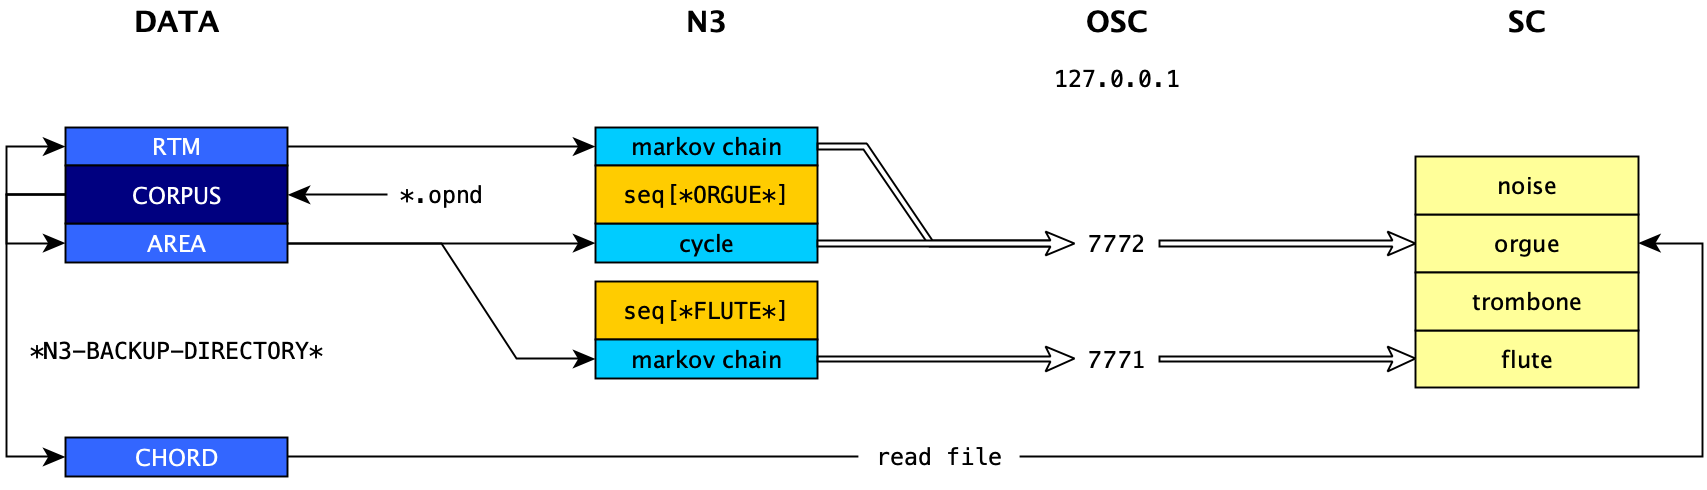
\includegraphics[width=\textwidth]{../img/9901}
\caption{Synoptic overview -- data $\rightarrow$ N3 $\rightarrow$ SC.}
\label{global}
\end{figure}

According to the synoptic overview on figure \ref{global}, we start from a corpus composed of sequences, which are composed of voices. Then, the parsing of the corpus encodes the duration, degree, and interval to the next note in the N3 AREA, which will learn voices by voices as monody. 

Second step, the rhythm of each voice is recorded in a file in order to be used as a corpus dataset of the sequencing in terms of probabilities.

Finally, the harmony context is parsed as a sequence of chords defined by the ordered degrees, in order to interact in the field of this harmony.

\bigskip

N3 as a connectionism network sent by OSC protocol a monophonic Markov chain, plus a combination of emergent cycles of the area.

SuperCollider receives and interprets OSC messages via a mixer (see figure \ref{iphonemix} on page \pageref{iphonemix}) where each instrument shares or conditions the data with the others (see figures \ref{deps} and  \ref{share}).

\begin{figure}[htbp]
\centering
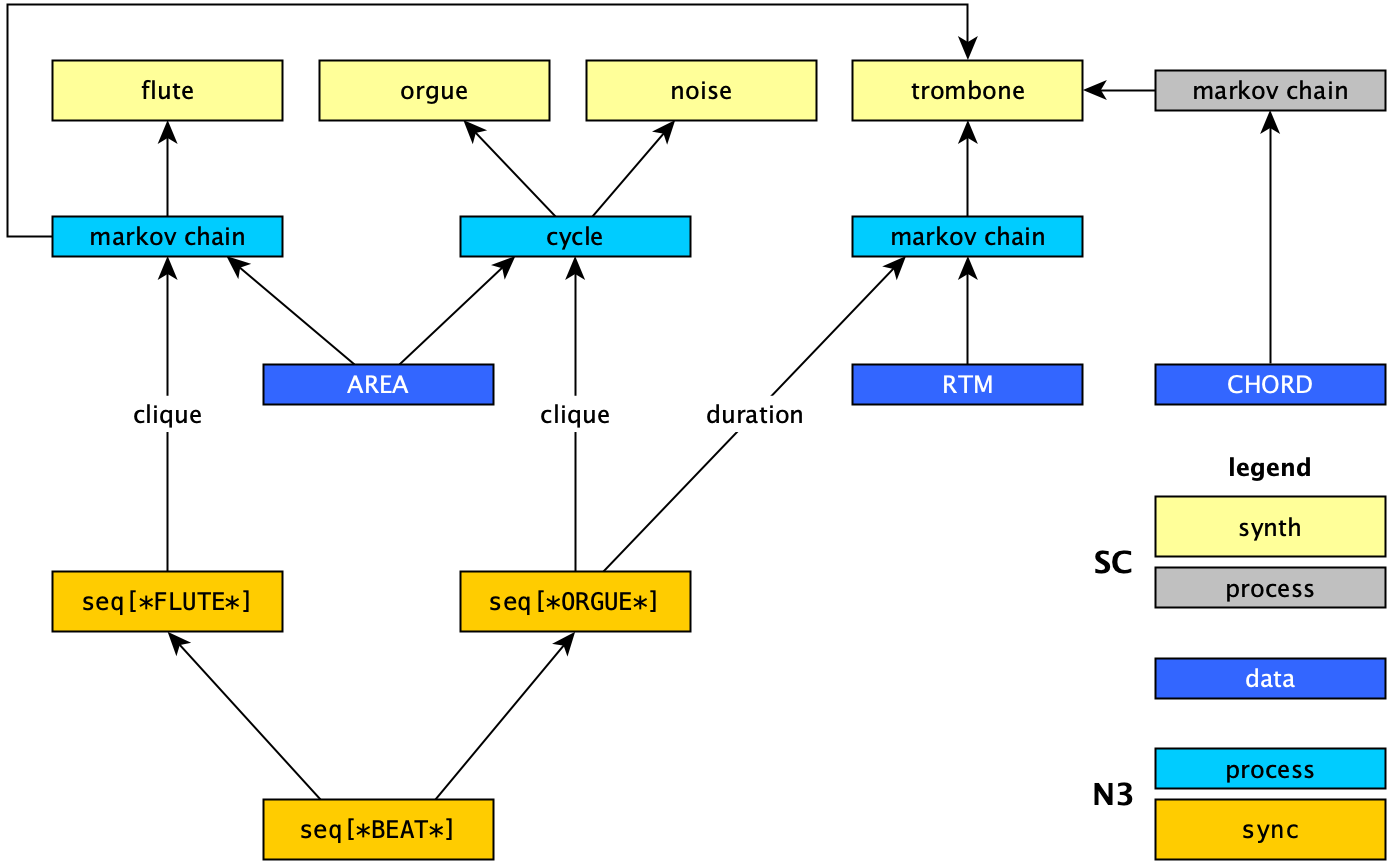
\includegraphics[width=\textwidth]{../img/9902}
\caption{Synoptic overview of the dependencies between components of the global process.}
\label{deps}
\end{figure}

\begin{figure}[htbp]
\centering
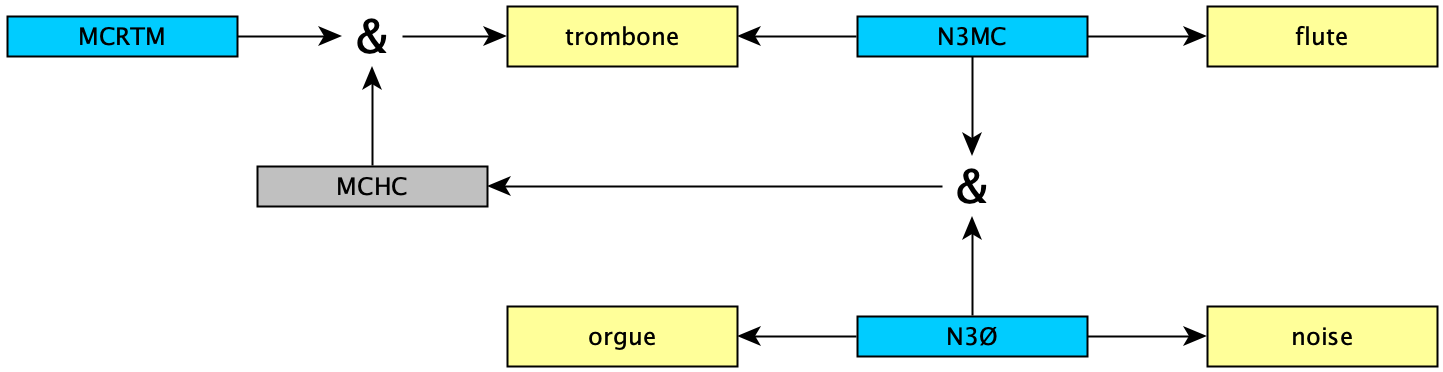
\includegraphics[width=\textwidth]{../img/9903}
\caption{Synoptic overview of which processes are involved at the synthesis level as arguments. \\ \textbf{Legend}:\\ -- \textsf{\footnotesize MCRTM} $\rightarrow$ markov chain according to the learned rhythms;\\ -- \textsf{\footnotesize N3Ø} $\rightarrow$ the emergent cycle of AREA;\\ -- \textsf{\footnotesize N3MC} $\rightarrow$ global AREA markov chain;\\ --   \textsf{\footnotesize MCHC} $\rightarrow$ markov chain according to the harmonic context.}
\label{share}
\end{figure}

\subsection{Learning  dataset}

Source\footnote{\href{http://www.titanmusic.com/data.php}{\texttt{\scriptsize http://www.titanmusic.com/data.php}}} ... First book of J. S. Bach's \textit{Das Wohltemperirte Klavier} (BWV 846 -- 869), 41544 notes ...
    
\begin{lstlisting}[language=N3]
N3>  (load-opt "OPND")
#P".../N3/opt/OPND"
N3> (defparameter +corpus+ 
 (loop 
   for file in 
    (directory ".../bach-database/ps13escomopnd/*-mel.opnd") 
;; for this corpus every 4 files the tonality increases by 1
;;  ---> (M prelude, M fugue, m prelude, m fugue)
;; so the floor function on 0.25 step allows to transpose 
;; all files by 4 to modulo 0 -- i.e. C    
   for tune from 0 by 0.25 
  collect (map-opnd file 
    :tune (floor tune)
    :out ".../chord.data")))  
+CORPUS+
#|
( ;; list of sequences
 ( ;; sequence_1
  ( ;; voice_1
   (dur_1 deg_1 int_1 chord_1)
   (dur_2 deg_2 int_2 chord_2)
   ...
   (dur_n deg_n int_n chord_n)
  )
 )
)
|#
;; format the file generated previously 
;; with the function map-opnd with the key :out
N3> (df2sc (".../chord.data"))
;; which generate the SuperCollider file
;; .../chord.scd 
;; setting ~chord in SuperCollider environment
;  ---> see harmonic context  voice 3
;------
;  --->  create and initiate area -- see annex 2.1 
;        with :cover-value 5 and :topology 3
; the +CORPUS+ should be a list of sequence of cliques
; then consider it as equal to (flat-once +corpus+)
;------
N3> (defparameter +rtm+ (flat-once (loop for seq in +corpus+ collect (loop for voice in seq when (butlast voice) collect (butlast (mapcar #'car voice))))))
+RTM+
#|
( ;; list of rtm by voice
 (rtm_seq_1_voice_1)
 (rtm_seq_1_voice_2)
 ...
 (rtm_seq_2_voice_1)
 ...
 (rtm_seq_n_voice_n)
)
|#
;  ---> see voices 2 and 3
; +RTM+ as `monnayage' of the voice 2 played by the voice 3
\end{lstlisting}

\bigskip

The retrieving learned sequences from the corpus, despite the `cover value' of 5, is not efficient enough because of the lack of discriminative parameter. Nevertheless, this study is rather focusing on an extreme minimalist approach than the ability to recognise sequence snippets from memory. Only, the matrix probabilities cannot reach 100\%, which is not  required because it is not question of quotation or reference of the acquired. Then it is currently question to (a) envisage the potential of this AI in context according to the acquired, and (b) to underlining potential issues, such as computation time and interactivity between voices. 

\begin{lstlisting}[language=N3]
N3> (save corpus)
\end{lstlisting}

\subsection{Sequencing instantiation}

\subsubsection{Voice 1}

Iniatialisation of the voice 1 as a physical modeling flute in SC. This instance generates a Markov chain sequence according to two simple rules such as the next degree is evaluated according to the previous interval and avoid more than 4 successive repetitions in term of duration. The number of repetitions can be modulated, as well as the pulse and the function of \texttt{:odds}.

\begin{lstlisting}[language=N3]
;;----------------------------------
(create-sequencing
 :net CORPUS
 :dub '*flute*
 :pulse 3
 :buffer-size 50
 :port 7771)
;;----------------------------------
; this rule set the degree of the next event 
; according to the interval of the current one.
(set-rule *flute* 
  (let ((nn (mod (+ (cadr (car (buffer-out self)))
		     ; minus 11 according to the encoding of intervals
		     (- (caddr (car (buffer-out self))) 11))
		     12)) ; modulo 12
	      ; no more than 4 repetitions duration allowed	 
	      (rep (remove-duplicates
	       (loop for i from 1 to 4 for c in (buffer-out self)
		     collect (car c)))))
    (if (singleton rep)
	     (list (caadr (pick-other-experience
		      (locate-clique corpus (list '? nn '?))
		      (list (car rep) nn '?))) nn '?)
	     (list '? nn '?))))
;; hack to add next event to the OSC message	
(setf (gethash 'ind (mem-cache *flute*)) :next)
;;----------------------------------
(set-routine *flute*   
  (markov-chain self :buffer (buffer-out self) 
    :odds #'max-weighted))
;;----------------------------------
(save *flute*)
\end{lstlisting}

\subsubsection{Voice 2}

Initialisation of the voice 2 as a kind of (original) organum in SC. This instance plays a pattern defined by interlacing emergent cycles for each MLT of the AREA.

Note that the rule as to return a \textit{clique} with or without the wild card '? (without in that case), and the routine fills the buffer with that \textit{clique} -- by computation in case of wild card. This can be done as an external function as  \texttt{markov-chain}, or like here by coding directly knowing that the current sequencing is called by the argument \textit{self}.

\bigskip

Alternative `routine' for the third voice as a sub-rhythm-pattern\footnote{Mint (`\textit{monnayage}'), i.e. a replacement of a term by several more brief ones and overall length equivalent; in other words fit the same duration. }
 according to the corpus (N3 side) and using the contextual harmony (SC  side) -- i.e. degrees of flute and orgue plus their respective intervals. The corpus is the list of the durations of each voice of each sequence from the initial corpus.
 
\begin{lstlisting}[language=N3]
;;----------------------------------
(create-sequencing
 :dub '*orgue*
 :pulse 1/3 ;; meaning a pulse of 3 beat hence the value of the meter must to be a multiple of (/ 1 pulse)
 :meter 12 
 :port 7772)
;;----------------------------------
;; set pattern
(require 'cl-cycle)
(set-pattern *orgue* (apply #'cl-cycle:interlace-cycle
    (loop for s in (soms-list corpus) collect
      (butlast (lst>trn (car (locate-cycle (id s))))))))	
;;----------------------------------		
;; load alternative rhythm corpus as `monnayage'
(set-corpus *orgue* +rtm+)
;; grab event in pattern 
(set-rule *orgue* 
  (let ((cli (nth (mod (gethash 'pattern-counter 
    (mem-cache self)) (length (pattern self))) 
      (pattern self)))
        (nextcli (nth (mod  (1+ (gethash 'pattern-counter 
    (mem-cache self))) (length (pattern self))) 
      (pattern self))))
;; compute rtm `monnayage'
  (append cli nextcli (list! (next-event-probability 
    (/ (1+ (car cli)) (* +beat+ (pulse self))) self 
    :opt :sum :remanence :corpus :result :eval 
    :compute #'min-weighted)))))
;;----------------------------------
 (set-routine *orgue* 
  (push (funcall (rule self) self) (buffer-out self))
  (incf (gethash 'pattern-counter (mem-cache self))))
;;----------------------------------
(save *orgue*)
\end{lstlisting}

\subsubsection{Voice 3}

The voice 3 as a physical modeling trombone (from FAUST\footnote{\href{https://faust.grame.fr/}{\texttt{\scriptsize https://faust.grame.fr/}}} library as \texttt{pm.brass\_ui} using \texttt{pm.brassModel}) in SC requires preliminary manipulation in order to define relevant descriptors in relation with its basics parameters (i.e. the pressure, the lips tension and the length of the tube).

\bigskip

Three parameters from the \textit{UGen} named \texttt{Brass} as:
\begin{itemize}
\item \texttt{pressure [0.1..1]}
\item \texttt{lips\_tension [0.1..1]}
\item \texttt{tube\_length [0.1..2.5]} (should be done or tested on 0.01 step as 1 cm, but this will increase exponentially the possibility and this against the CPU and RAM resources)
\end{itemize}

\bigskip

One (plus one as reliability) from also SC with the \textit{UGen} \texttt{Pitch}:
\begin{itemize}
\item \texttt{pitch [freq$|$reliability]}
\end{itemize}

\bigskip

And three more parameters (plus two as reliability) from the Praat analysis thanks to the preliminary analysis of the loudness profile and Common Lisp for the computation (see command line \textsl{enkode} with the option \texttt{-se} --  version 7.0) in order to detect emergent frequency -- as a kind of roughness indicator -- from the peaks of the said loudness profile; the reliability is the standard deviation of the normalised values subtracted to one:
\begin{itemize}
\item \texttt{roughness [freq$|$reliability]} 
\item \texttt{loudness [sone$|$reliability]} (of the emergent frequency)
\item \texttt{intensity [dB]} (of the sample)
\end{itemize}

\smallskip

More details about procedures, scripts and parameters in the SuperCollider  \texttt{tbn2CSV.scd} file, plus annexes page \pageref{annexes}, plus FAUST as \texttt{SynthDef \textbackslash tbn} in \texttt{synths.scd} file.

\bigskip

On the SuperCollider side, -- according to the the switching values of \textsf{flute/orgue} ($\blacksquare/\square$) and \textsf{RTM\_(on/off)} ($\blacksquare/\square$) buttons on the SC gui -- the trombone plays the following:
\begin{itemize}
\item[$\blacksquare\square$] \textsf{flute/RTM\_off} -- unison/octave of the flute;
\item[$\square\square$] \textsf{orgue/RTM\_off} -- unison/octave of the orgue with the rhythm of the flute;
\item[$\square\blacksquare$] \textsf{orgue/RTM\_on} -- unison/octave of the orgue with its own `mint' rhythm;
\item[$\blacksquare\blacksquare$] \textsf{flute/RTM\_on} -- harmonic context of the flute and the orgue with its own `mint' rhythm. The harmonic context is evaluated according to the data file \textsf{chord.scd} (see comment in the Chapter \textsl{Learning dataset}) as a dynamic Markov chain with the class \texttt{MarkovSet}\footnote{\href{https://github.com/yannics/MathLib/tree/yannics-patch-1}{\texttt{\scriptsize https://github.com/yannics/MathLib/tree/yannics-patch-1}}} (see details in documentation of this class plus comment SC file).
\end{itemize}

\subsubsection{Voice 4}

The fourth voice consists to grab the pitch and incidentally the rhythm of the \texttt{*orgue*} in order to `granulate' by stepping frames through one sample, previously created for analysis, of the trombone. Each sample is selected according to its pitch as degree followed by its related pitch defined by its interval (at half time of the duration) matching \texttt{(60..72).midicps} as indices. (this does not affect the result as such, but allows to renew the sample according to some logical context). 

\subsubsection{Voice 5}

The pitches of the \texttt{*orgue*} are interpreted with the \textit{pseudo-UGen} \texttt{Ulam} 
(See 7.6 in \textsl{Journal of Generative Sonic Art} [Ics 2014/24]).%\citep{yi}).

The \texttt{Ulam}'s parameters are:
\begin{description}
\item[\quad ar] -- an \myuline{array of frequencies} correlated with the current degree of the \texttt{*orgue*}: \texttt{($\sim$frequencies/$\sim$frequencies.minItem).round(0.01)\\
 * (60..72).midicps[$\sim$degOrg]}
\item[\quad ind] -- $\sim$\texttt{modeUlam} (0 by default -- \textit{i.e.} \textsf{reson} and 1 for \textsf{sine} -- as sound generator)
\item[\quad stretch] $\sim$\texttt{tpsOrg} as \myuline{duration} of the event.
\item[\quad [ \textit{nx}] -- \textit{$0$ default value (fit the collatz profile into the duration)} \textbf{]}
\item[\quad [ \textit{ny}] -- \textbackslash\texttt{max} \textit{default value (normalize the collatz profile with its max value)} \textbf{]}
\item[\quad [ \textit{sig}] -- \textbackslash\texttt{norm} \textit{default value (normalize the output signal between $-1$ and $1$)} \textbf{]}
\item[\quad detune] -- $\sim$\texttt{detune} (5) -- detune randomly between $-5$ and $5$ Hz each frequency of the input array of frequencies
\item[\quad rndAmp] -- $\sim$\texttt{rndAmp} (0.1) -- each collatz profile as signal is multiplied by a random value between $0.1$ and $1$
\end{description}

\subsubsection{Synchronization}

Silent (i.e. no specific data) sequencing as a tempo indicator or as a background mouvement, marking pulses, beats, and measures. 

\begin{lstlisting}[language=N3]
;;----------------------------------
(create-sequencing :dub '*beat* :port 7000)
;;----------------------------------
(set-rule *beat*
  (if (buffer-out self)
   (gethash 'generic-counter (mem-cache self))
   (setf (gethash 'generic-counter (mem-cache self))
	 (list
	     0 ;; as indice of the minimal relative duration
	       ;; in other word 1 pulse
	     1 ;; pulse counter   (1)
	     (pulse self)
	     1 ;; beat counter    (3)
	     (meter self)
	     1 ;; measure counter (5)
	     ))))
;;----------------------------------	     
(set-routine *beat* 
  (push (funcall (rule self) self) (buffer-out self))
  (let ((cbuf 
  (copy-list (gethash 'generic-counter (mem-cache self)))))
    (if (>= (nth 1 cbuf) (pulse self))
       (progn
          (incf (nth 3 cbuf))
          (setf (nth 1 cbuf) 1))
       (incf (nth 1 cbuf)))
    (when (> (nth 3 cbuf) (meter self))
      (incf (nth 5 cbuf))
      (setf (nth 3 cbuf) 1))
   (setf (gethash 'generic-counter (mem-cache self)) cbuf)))
;;----------------------------------
(save *beat*)
\end{lstlisting}

\begin{lstlisting}[language=N3,basicstyle=\ttfamily\footnotesize]
;; synchronize with the previous sequencing
N3> (set-sync *flute* *beat* :save t)
|          | sequencing | pulse | meter | sync   | anacrusis |
| -------- | ---------- | ----- | ----- | ------ | --------- |
| LEADER   | *BEAT*     |     4 |     8 | NIL    |         0 |
| FOLLOWER | *FLUTE*    |     3 |     4 | *BEAT* |         0 |
NIL
N3> (set-sync *orgue* *beat* :save t)
|          | sequencing | pulse | meter | sync   | anacrusis |
| -------- | ---------- | ----- | ----- | ------ | --------- |
| LEADER   | *BEAT*     |     4 |     8 | NIL    |         0 |
| FOLLOWER | *ORGUE*    |   1/3 |    12 | *BEAT* |         0 |
NIL
\end{lstlisting}

\subsection{Third-parties}
\addtocounter{footnote}{-2}

To connect any third-part, this is done through the cache memory defined by the keyword \texttt{thirdpart}, as a list of \texttt{lambda*} function. 

\begin{lstlisting}[language=N3]
;; loading thirdpart 
(load-opt "thirdpart")
;; enable thirdpart
(setf *thirdpart* t)
\end{lstlisting}

\begin{figure}[h]
\centering
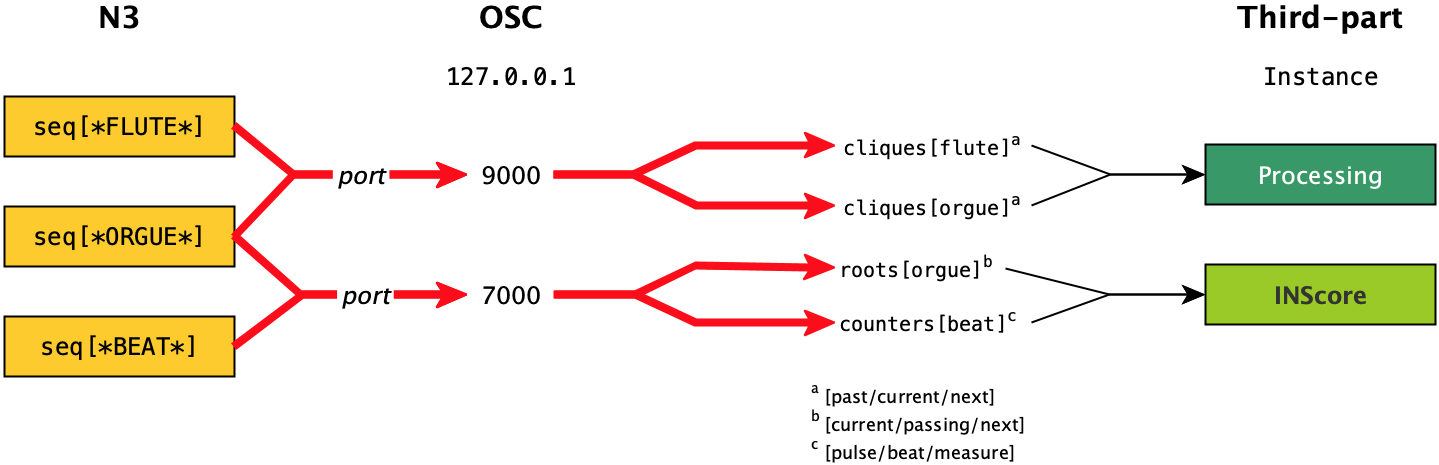
\includegraphics[width=\textwidth]{../img/9910}
\caption{Third parties OSC communication overview as instances, from N3 sequencing to Processing\protect\footnotemark \, and INScore\protect\footnotemark.}
\end{figure}
\addtocounter{footnote}{-1}
\footnotetext{\href{https://processing.org}{\texttt{\scriptsize https://processing.org}}}  
\stepcounter{footnote}
\footnotetext{\href{https://inscore.grame.fr}{\texttt{\scriptsize https://inscore.grame.fr}}}  

\subsubsection{Initialisation}

This is writing a data file for Processing, as in this case the position of all fanals of an AREA. 
\begin{lstlisting}[language=N3]
;; init Processing data
N3> (init-process corpus "~/Documents/Processing/N3_P5")
\end{lstlisting}

\subsubsection{Sending message}

The OSC message sent to Processing is formatted as follow:

\smallskip

 \texttt{\small [voice, rdur-1, deg-1, int-1, rdur, deg, int, rdur+1, deg+1, int+1]}
 
 \smallskip
 
Which means \texttt{voice} as an id (1 for the flute [clique as the clear triangle], and 2 for the orgue [clique as red triangle]), \texttt{rdur} as the relative duration, \texttt{deg} as the degree, and \texttt{int} as the interval to the potential next note, as respectively the previous clique (minus one), the current clique, and the next clique (plus one).

\begin{figure}[h]
\centering
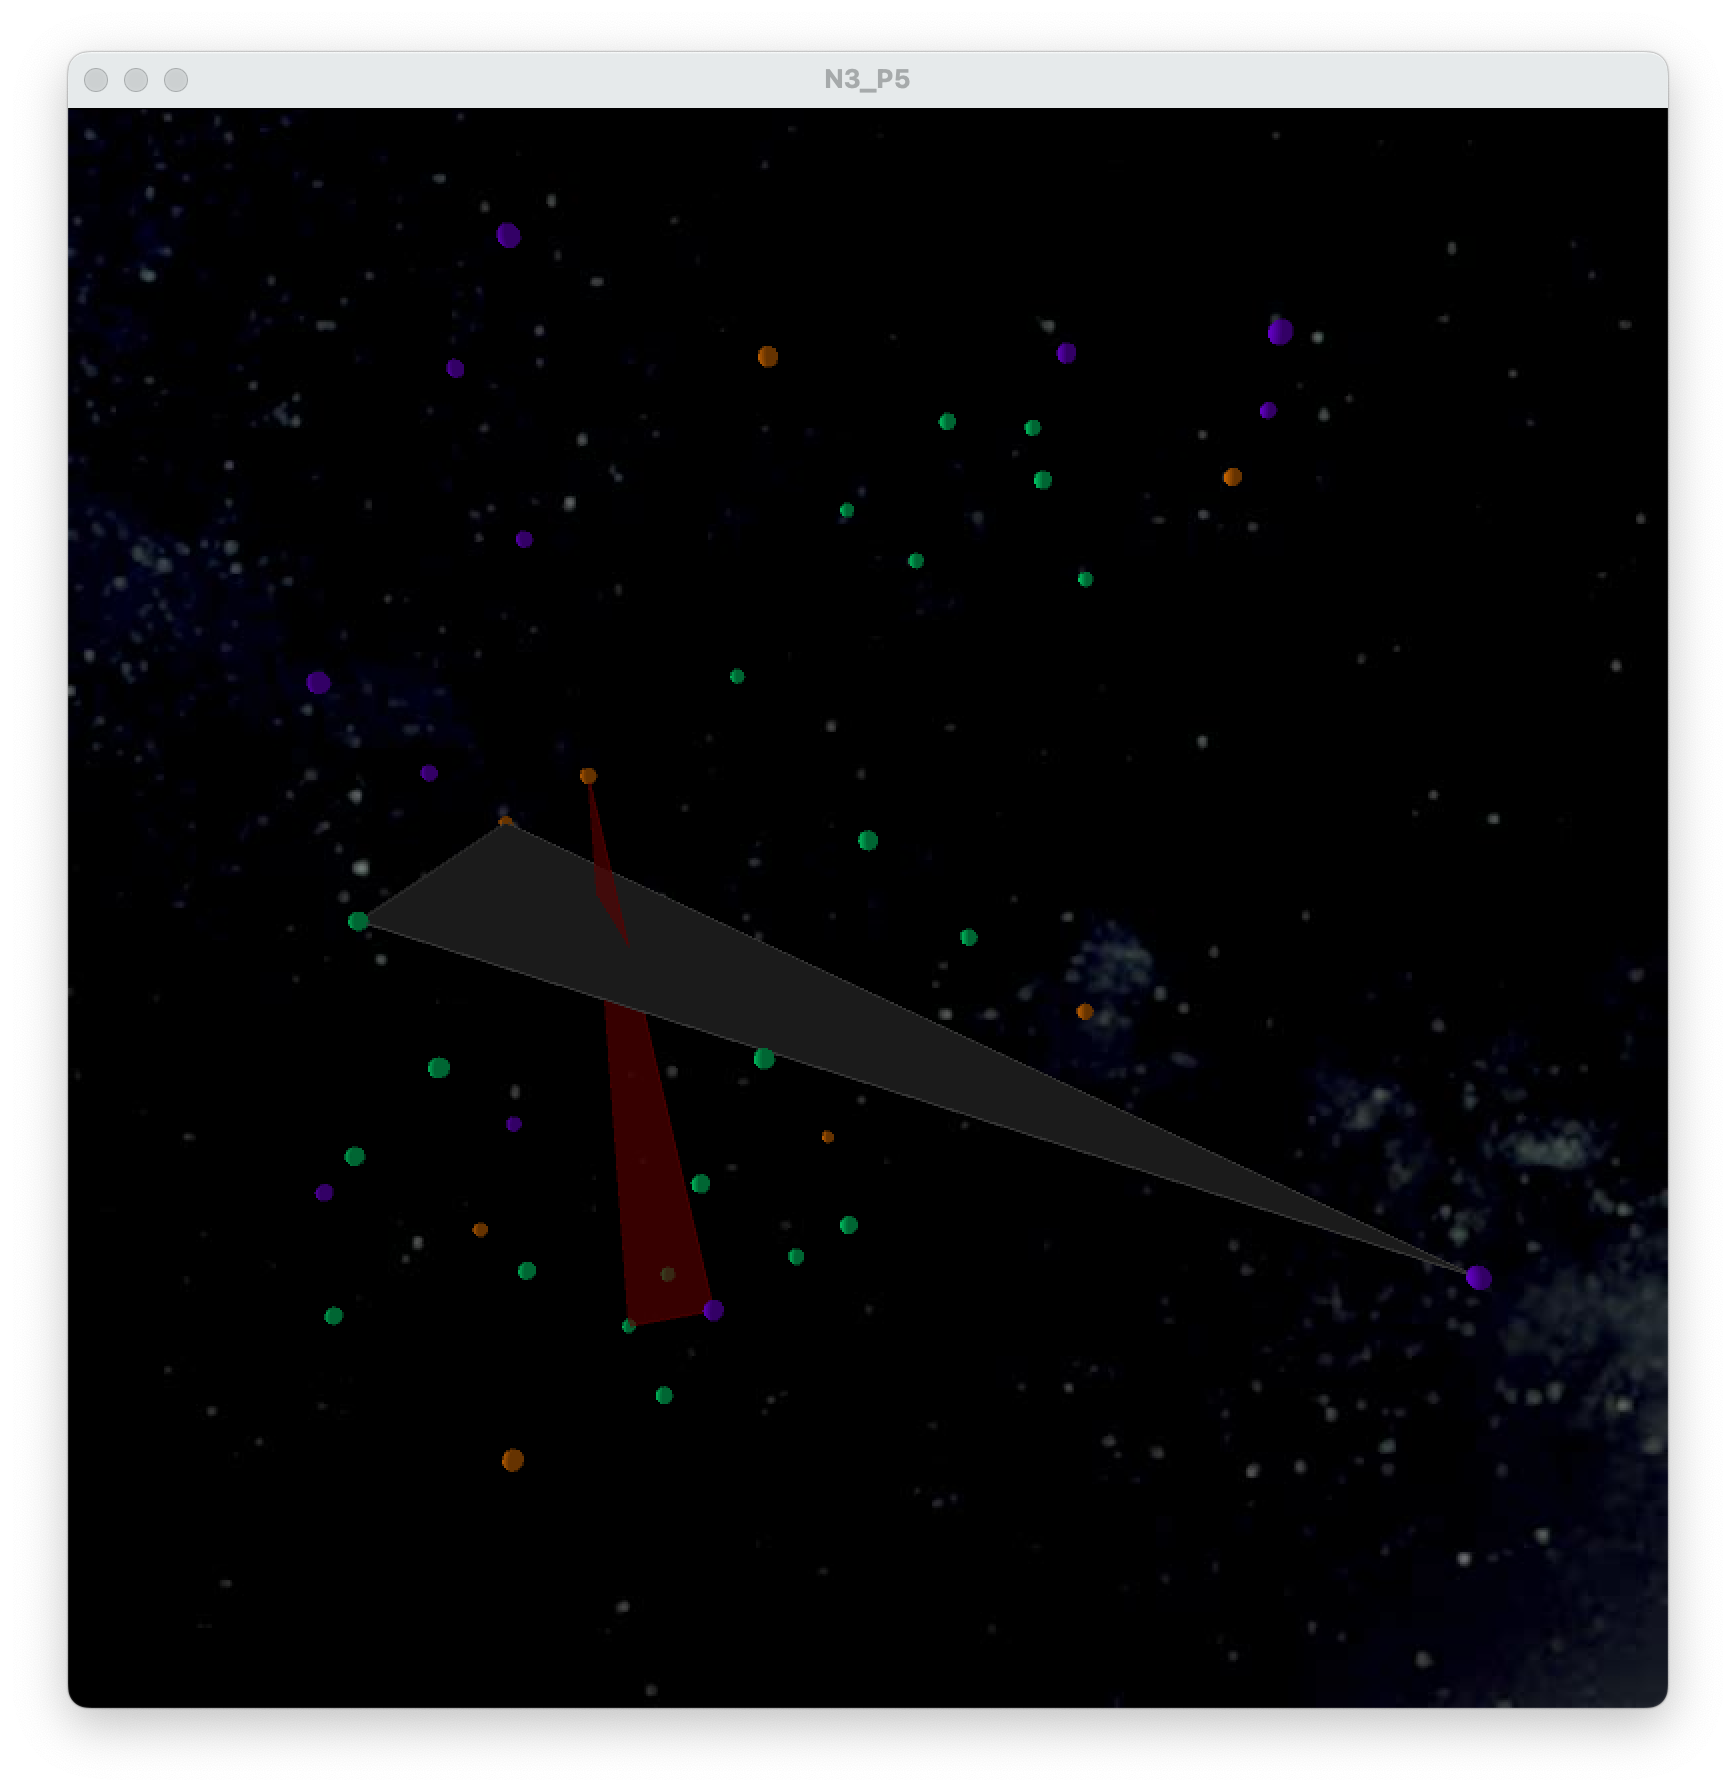
\includegraphics[width=\textwidth]{../img/9920}
\caption{This is a 3D representation of the AREA network CORPUS. The `planets' are the `fanals' for each MLT of the AREA, respectively orange for relative durations, blue for degrees, and green for intervals.}
\end{figure}

Note the previous and the next cliques are not yet displayed on Processing, because of the how to do that in a readable manner (work in progress...). 

\begin{lstlisting}[language=N3]
;;----------------------------------
;; Voice 1 [*flute*]
;; OSC message to Processing (port 9000)
(thirdpart-message 
  (lambda* (self)
    (send-udp
      (cons "/sc3p5"
        (append
           '(1) ;; voice id
		       ;; previous clique
		       (if (gethash 'last-event (mem-cache self))
		         (car (gethash 'last-event (mem-cache self)))
		         (carlast (buffer-out self)))
		       ;; current clique 
		       (carlast (buffer-out self))
		       ;; next clique 
		       (cadr (reverse (buffer-out self)))))
	  "127.0.0.1" 9000)))
\end{lstlisting}
\begin{lstlisting}[language=N3]
;;----------------------------------
;; Voice 2 [*orgue*]
;; OSC message to Processing (port 9000)
(thirdpart-message
  (lambda* (self)
    (send-udp
     (cons "/sc3p5"
       (append
         '(2) ;; voice id
         ;; previous clique
         (if (gethash 'last-event (mem-cache self))
          (n-first 3 (car (gethash 'last-event (mem-cache self))))
          (n-first 3 (carlast (buffer-out self))))
         ;; current clique 
         (n-first 3 (carlast (buffer-out self)))
         ;; next clique 
         (n-first 3 (cadr (reverse (buffer-out self))))))
	  "127.0.0.1" 9000)))
\end{lstlisting}

\subsection{Playing time}

\begin{lstlisting}[language=N3]
;;----------------------------------
(require 'N3)
;; loading AREA and SEQUENCING
(progn
  (load-neural-network "CORPUS")
  (load-sequencing "beat")
  (load-sequencing "flute")
  (load-sequencing "orgue"))
;; ... and play
(progn
  (act-routine *beat*)
  (act-routine *orgue*)
  (act-routine *flute*))
;; ... and stop
(progn
  (kill-routine *flute*)
  (kill-routine *orgue*)
  (kill-routine *beat*))
;;----------------------------------
\end{lstlisting}

The mixing stage is ensured on a iphone thanks to the app TouchOSC Mk1\footnote{\href{https://hexler.net/touchosc-mk1}{\texttt{\scriptsize https://hexler.net/touchosc-mk1}}}.

\begin{figure}[H]
\centering
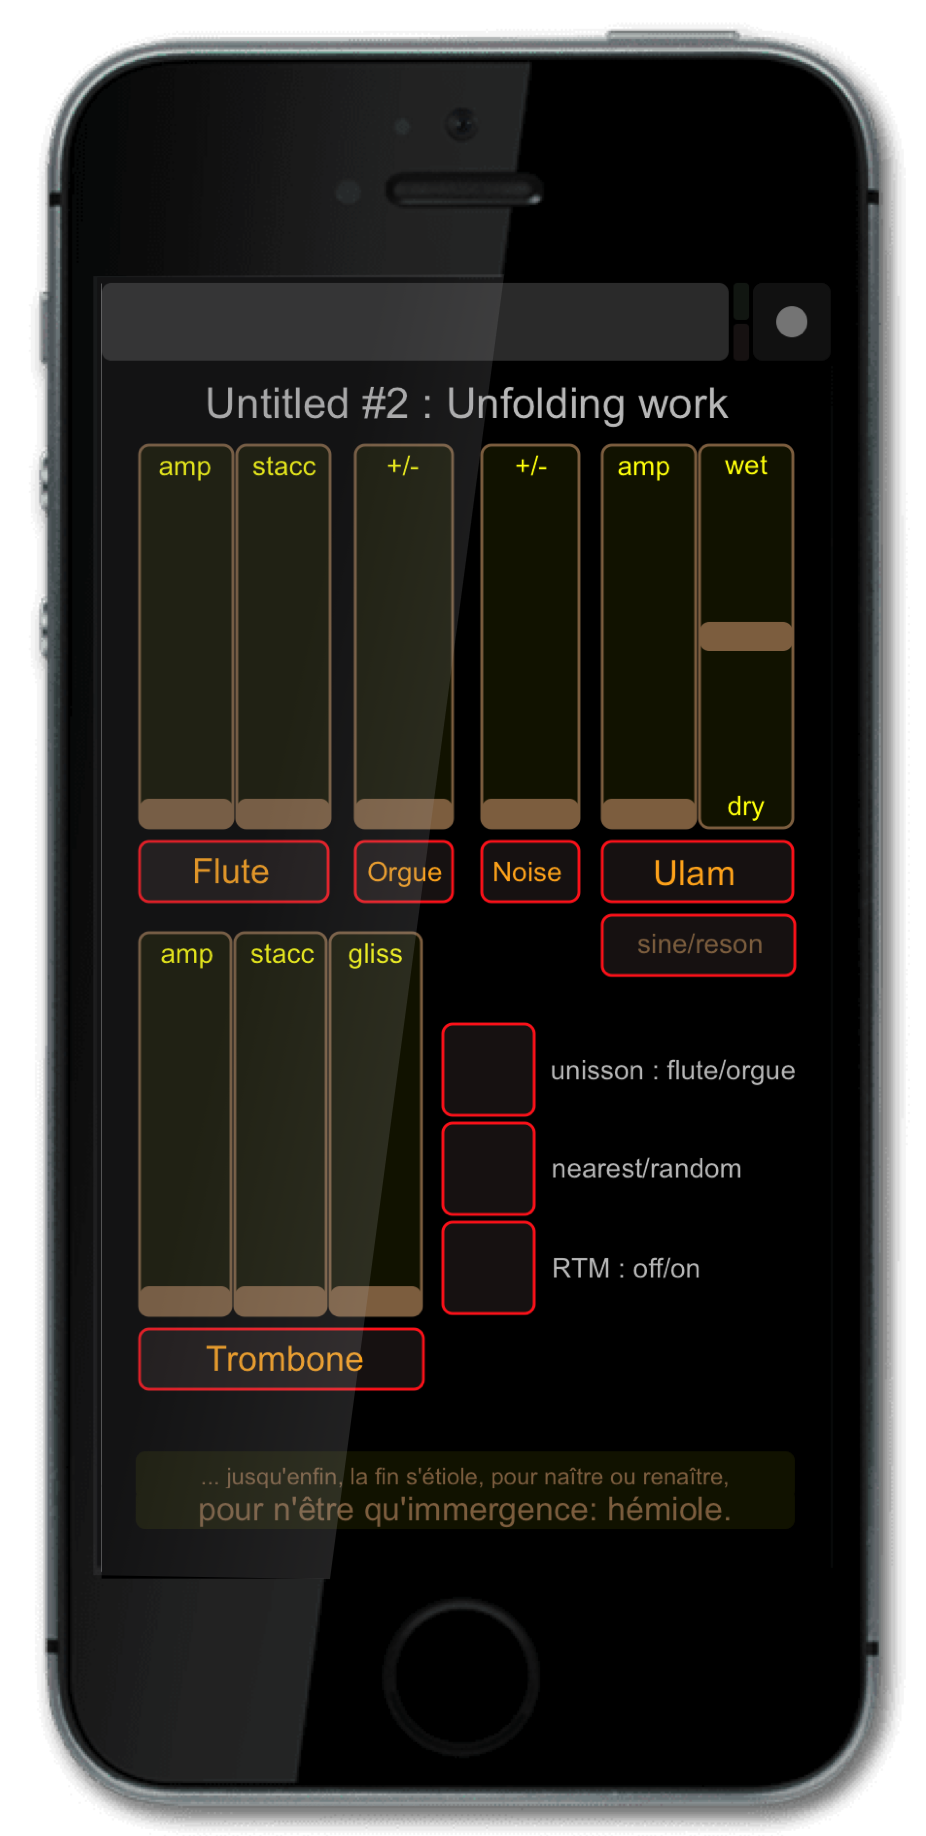
\includegraphics[width=\textwidth/2]{../img/9930}
\caption{TouchOSC Mk1 layout for mixing.}
\label{iphonemix}
\end{figure}

\newpage

\section*{Annexes}
\label{annexes}

\subsection*{...}

\begin{figure}[H]
\centering
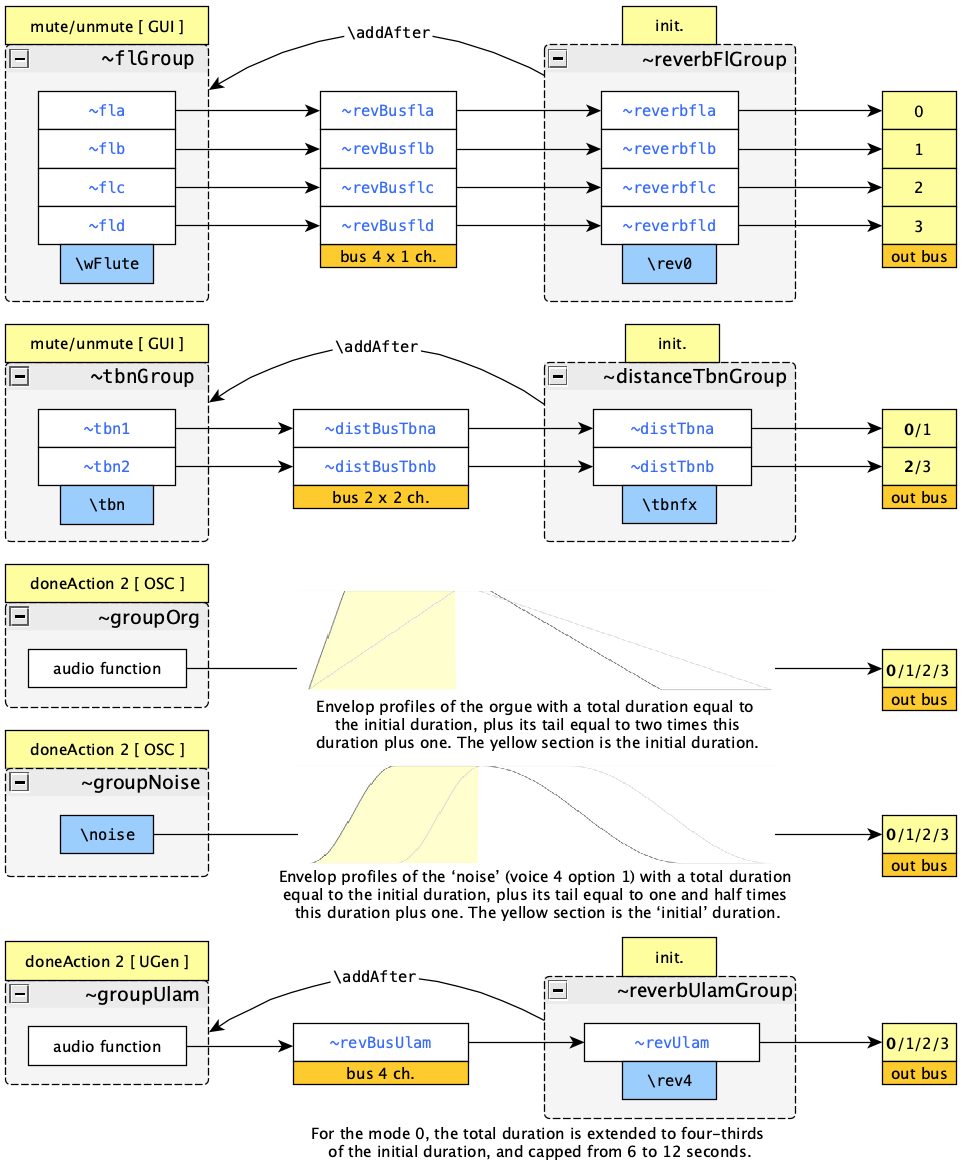
\includegraphics[width=\textwidth-1mm]{../img/9940}
%\caption{...}
\label{struc}
\end{figure}

\newpage
\subsection*{Psychoacoustics -- Roughness}

See Ics Y. \textit{Journal of Generative Sonic Art} (2014/\the\year), Section 1.8.\\ Online at: \href{https://www.overleaf.com/read/sjhfhthgkgdj}{\texttt{\small https://www.overleaf.com/read/sjhfhthgkgdj}} [Accessed \today]

\bigskip

Source:  University of Salford Manchester 

\noindent \href{https://hub.salford.ac.uk/sirc-acoustics/psychoacoustics/sound-quality-making-products-sound-better/an-introduction-to-sound-quality-testing/roughness-fluctuation-strength/}{\texttt{\small https://hub.salford.ac.uk/sirc-acoustics/psychoacoustics/sound-quality-\\ \noindent making-products-sound-better/an-introduction-to-sound-quality-testing/\\ \noindent roughness-fluctuation-strength/}}

\subsubsection*{Next pages}

Zwicker E., Fastl H. \textit{Psychoacoustics: Facts and Models} (1990), pp. 247--264.

\includepdf[pages={5-22},scale=.8]{Psychoacoustics_Facts_and_Models_----_(Pages_251_to_275).pdf}

\end{document}